\begin{comment}
\documentclass[10pt]{article}
\usepackage{fullpage, graphicx, url}
\setlength{\parskip}{1ex}
\setlength{\parindent}{0ex}
\title{FLpanel}
\begin{document}


\begin{tabular}{ccc}
The Alternative Csound Reference Manual & & \\
Previous & &Next

\end{tabular}

%\hline 
\end{comment}
\section{FLpanel}
FLpanel�--� Creates a window that contains FLTK widgets. \subsection*{Description}


  Creates a window that contains FLTK widgets. 
\subsection*{Syntax}


 \textbf{FLpanel}
 ``label'', iwidth, iheight [, ix] [, iy] [, iborder]
\subsection*{Initialization}


 \emph{``label''}
 -- a double-quoted string containing some user-provided text, placed near the corresponding widget. 


 \emph{iwidth}
 -- width of widget. 


 \emph{iheight}
 -- height of widget. 


 \emph{ix}
 (optional) -- horizontal position of upper left corner of the valuator, relative to the upper left corner of corresponding window (expressed in pixels). 


 \emph{iy}
 (optional) -- vertical position of upper left corner of the valuator, relative to the upper left corner of corresponding window (expressed in pixels). 


 \emph{iborder}
 (optional) -- border type of the container. It is expressed by means of an integer number chosen from the following: 


 
\begin{itemize}
\item 

 0 - no border

\item 

 1 - down box border

\item 

 2 - up box border

\item 

 3 - engraved border

\item 

 4 - embossed border

\item 

 5 - black line border

\item 

 6 - thin down border

\item 

 7 - thin up border


\end{itemize}
\subsection*{Performance}


  Containers are useful to format the graphic appearance of the widgets. The most important container is \emph{FLpanel}
, that actually creates a window. It can be filled with other containers and/or valuators or other kinds of widgets. 


  There are no k-rate arguments in containers. 


 \emph{FLpanel}
 creates a window. It must be followed by the opcode \emph{FLpanelEnd}
 when all widgets internal to it are declared. For example: 


 
\begin{lstlisting}
        FLpanel   "PanelPluto",450,550,100,100 ;***** start of container
gk1,ih1 FLslider  "FLslider 1", 500, 1000, 2 ,1, -1, 300,15, 20,50
gk2,ih2 FLslider  "FLslider 2", 300, 5000, 2 ,3, -1, 300,15, 20,100
gk3,ih3 FLslider  "FLslider 3", 350, 1000, 2 ,5, -1, 300,15, 20,150
gk4,ih4 FLslider  "FLslider 4", 250, 5000, 1 ,11,-1, 300,30, 20,200
        FLpanelEnd ;***** end of container
        
\end{lstlisting}


 
 will output the following result: 

 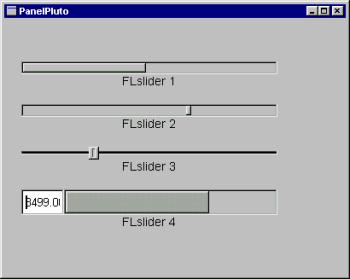
\includegraphics[scale=1]{flpanel} 


 FLpanel.
\subsection*{Examples}


  Here is an example of the flpanel opcode. It uses the files \emph{flpanel.orc}
 and \emph{flpanel.sco}
. 


 \textbf{Example 1. Example of the flpanel opcode.}

\begin{lstlisting}
/* flpanel.orc */
; Creates an empty window panel
sr = 44100
kr = 441
ksmps = 100
nchnls = 1

; Panel height in pixels
ipanelheight = 900
; Panel width in pixels
ipanelwidth = 400
; Horizontal position of the panel on screen in pixels
ix = 50
; Vertical position of the panel on screen in pixels
iy = 50

FLpanel "A Window Panel", ipanelheight, ipanelwidth, ix, iy
; End of panel contents
FLpanelEnd

;Run the widget thread!
FLrun

instr 1
endin
/* flpanel.orc */
        
\end{lstlisting}
\begin{lstlisting}
/* flpanel.sco */
; 'Dummy' score event of 1 hour.
f 0 3600
e
/* flpanel.sco */
        
\end{lstlisting}
\subsection*{See Also}


 \emph{FLgroup}
, \emph{FLgroupEnd}
, \emph{FLpack}
, \emph{FLpackEnd}
, \emph{FLpanelEnd}
, \emph{FLscroll}
, \emph{FLscrollEnd}
, \emph{FLtabs}
, \emph{FLtabsEnd}

\subsection*{Credits}


 Author: Gabriel Maldonado


 New in version 4.22


 Example written by Iain McCurdy, edited by Kevin Conder.
%\hline 


\begin{comment}
\begin{tabular}{lcr}
Previous &Home &Next \\
FLpackEnd &Up &FLpanelEnd

\end{tabular}


\end{document}
\end{comment}
